\section{Fundamentos} 

\begin{enumerate}[label=\textbf{\arabic*.}, ref=\arabic*]
    \item\textsuperscript{*} Exiba a fronteira do conjunto $\{d_{0},d_{1},d_{3}\}$ no grafo da direita do Exercício 8. 

    \noindent \textbf{Resolução:} \\
    A fronteira do conjunto $X = \{d_0, d_1, d_3\}$ é dada por:
    \[
    \partial(X) = \{c_1, c_2, c_4, c_5, d_2\}
    \]
    \textbf{Justificativa:} Por definição, a fronteira de um conjunto consiste nos vértices adjacentes aos elementos de $X$ que não pertencem ao próprio $X$.
    
    \item\textsuperscript{*} Quantas arestas tem um grafo completo de $n$ vértices? Justifique sua resposta. 
    
    \noindent \textbf{Resolução:}\\
    Por definição, um grafo completo é aquele em que cada vértice é vizinho de todos os outros, o equivalente a dizer que existe uma aresta entre cada par de vértices distintos. Pensei em duas maneiras distintas de resolver essa questão:
    
    \vspace{0.3cm}
    \noindent \textbf{i) Por combinatória:}\\
    Como existe exatamente uma aresta para toda dupla de vértices, a quantidade total de arestas é igual ao número de subconjuntos de tamanho 2 que podemos formar a partir do conjunto de $n$ vértices:
    \[
    |E(G)| = \left| \binom{V(G)}{2} \right| = \binom{|V(G)|}{2} = \binom{n}{2} = \frac{n(n-1)}{2}
    \]
    
    \vspace{0.3cm}
    \noindent \textbf{ii) Por matriz de adjacência:}\\
    Usando a representação por matriz de adjacência $M$ de dimensão $n \times n$ para um grafo completo, todos os valores fora da diagonal principal devem ser iguais a $1$, e os elementos da diagonal principal iguais a $0$ (já que não há laços).
    \[
    M = \begin{bmatrix}
    0 & 1 & 1 & \cdots & 1 \\
    1 & 0 & 1 & \cdots & 1 \\
    1 & 1 & 0 & \cdots & 1 \\
    \vdots & \vdots & \vdots & \ddots & \vdots \\
    1 & 1 & 1 & \cdots & 0
    \end{bmatrix}_{n \times n}
    \]
    Pelo Teorema 3, sabemos que a soma dos graus de todos os vértices de um grafo é o dobro do número de arestas:
    \[
    \sum_{v \in V(G)} \delta_G(v) = 2|E(G)|
    \]
    A soma dos graus corresponde à soma de todos os elementos da matriz de adjacência. Como a matriz possui $n \times n = n^2$ elementos no total e $n$ zeros na diagonal principal, a soma de todos os elementos é $n^2 - n$. Logo:
    \[
    2|E(G)| = n^2 - n \implies |E(G)| = \frac{n^2 - n}{2} = \frac{n(n-1)}{2}
    \]
    
    \item\textsuperscript{*} Se um vértice tem $k$ vizinhos em $G$, quantos vizinhos ele tem em $\overline{G^{\prime}}$? Justifique sua resposta. 

    \noindent \textbf{Resolução:}\\
    Por definição, o complemento de um grafo $G$ é o grafo $\overline{G}$ tal que $V(\overline{G}) = V(G)$ e $E(\overline{G}) = \binom{V(G)}{2} - E(G)$.
    
    Ou seja, para um vértice $v \in V(G)$ com $k$ vizinhos em $G$, existem $|V(G)| - 1$ outros vértices possíveis com os quais $v$ pode se conectar (pois excluímos o próprio $v$, já que não há laços). Desses possíveis vizinhos, $v$ já é adjacente a $k$ vértices. Portanto, os vértices não adjacentes a $v$ em $G$ somam $|V(G)| - 1 - k$.
    
    No grafo complemento $\overline{G}$, as adjacências se invertem: os vértices que não eram adjacentes passam a ser, e os $k$ que eram deixam de ser. Logo, o grau do vértice $v$ em $\overline{G}$ será:
    \[
    \delta_{\overline{G}}(v) = |V(G)| - 1 - k
    \]
    Essa é a quantidade de vizinhos de $v$ no grafo $\overline{G}$.

    
    \item\textsuperscript{*} Quantos grafos diferentes existem com o conjunto de vértices $\{1,...,n\}$? Justifique. 

    \noindent \textbf{Resolução:}
    
    \vspace{0.2cm}
    \noindent \textbf{i) Por combinatória:} fixando o conjunto dos vértices como $\{1,\dots,n\}$, o que vai diferenciar um grafo do outro é o conjunto de arestas. Ou seja, queremos saber quantos subconjuntos de arestas são possíveis. O grafo completo de $n$ vértices possui $\binom{n}{2}$ arestas. Portanto:
    $$| 2^{E(G)} | = \left| 2^{\binom{V(G)}{2}} \right| = 2^{\binom{n}{2}} = 2^{\left[ \frac{n(n-1)}{2} \right]}$$
    
    \vspace{0.2cm}
    \noindent \textbf{ii) Por matriz de adjacência:} Na representação por matriz de adjacência $n \times n$, temos que a diagonal principal é $0$ (não tem laços) e a matriz é simétrica (o grafo não é direcional). Portanto temos $\frac{n \times n - n}{2}$ quadradinhos para preencher com $0$ ou $1$. Pelo princípio multiplicativo, temos $2^{\left[ \frac{n(n-1)}{2} \right]}$ possibilidades.

    \item\textsuperscript{\#} Seja $G$ um grafo. Dados $X\subseteq V(G)$ e $n\in\mathbb{N}$ vamos definir $\Gamma_{G}^{n}(X)$ como segue. 
    
    \begin{equation*}
    \Gamma_{G}^{n}(X):=\begin{cases}X,& \text{se } n=0.\\ \Gamma_{G}(\Gamma_{G}^{n-1}(X)),& \text{se } n>0.\end{cases} 

    \end{equation*}
    \begin{enumerate}
        \item Exiba os conjuntos $\Gamma_{G}^{n}(\{a_{0},b_{2}\})$ para $n\in\{1,2,3,4,5\}$ onde $G$ é o grafo da esquerda no Exercício 8. 
        \item É verdade que para qualquer grafo $G$ e qualquer conjunto $X$ de seus vértices, existe um valor de $n\in\mathbb{N}$ tal que $\Gamma_{G}^{n}(X)=V(G)$? Justifique. 
        
        \item É verdade que para qualquer grafo $G$ e qualquer conjunto $X$ de seus vértices, existe um valor de $n\in\mathbb{N}$ tal que $\Gamma_{G}^{n}(X)=\Gamma_{G}^{n+1}(X)$? Justifique. 
        
    \end{enumerate}
    
    \item\textsuperscript{*} Seja $\mathcal{F}=\{A_{1},...,A_{n}\}$ uma família de subconjuntos de um conjunto $A$. O grafo de interseção de $\mathcal{F}$ é o grafo $\mathcal{I_{F}}$ dado por 
    
    $V(\mathcal{I_{F}}):=\mathcal{F},$ 
    
    $E(\mathcal{I}_{\mathcal{F}}):=\{\{A_{i},A_{j}\}|A_{i}\cap A_{j}\ne\emptyset\}$. 
    
    \begin{enumerate}
        \item Seja $G$ o grafo interseção de $\binom{\{1,...,5\}}{2}$. Desenhe $G$. 
        \item Desenhe $\overline{G}$ 
        
        \item Verifique que $\overline{G}$ (isomorfo a)o Grafo de Petersen. 
    \end{enumerate}
    
    \item\textsuperscript{*} Um grafo $G$ é um grafo de intervalo se é o grafo de interseção de um conjunto de intervalos fechados de $\mathbb{R}$. 
    \begin{enumerate}
        \item Os grafos $G_{1}$ e $G_{2}$ abaixo são grafos de intervalo? Justifique. 
        
        \begin{figure}[h]
            \centering 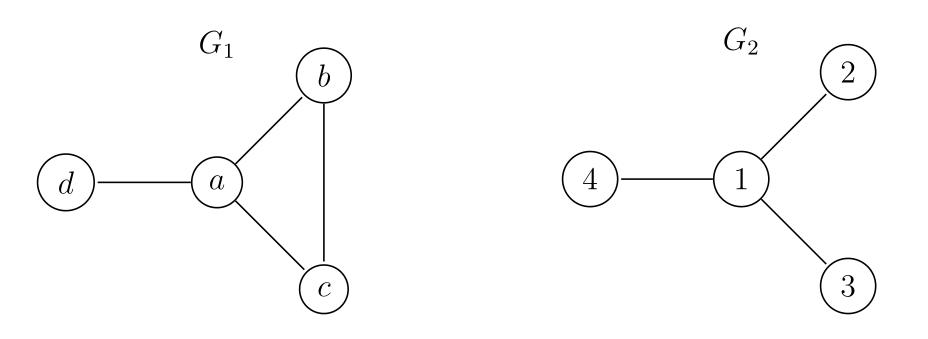
\includegraphics[width=0.8\textwidth]{q7.png}
        \end{figure}
        
        \item Dê um exemplo de um grafo que não é grafo de intervalo e prove que seu exemplo está correto.
    \end{enumerate}
    
    \item\textsuperscript{*} Prove que os grafos abaixo são isomorfos. 
    \begin{figure}[h]
        \centering
        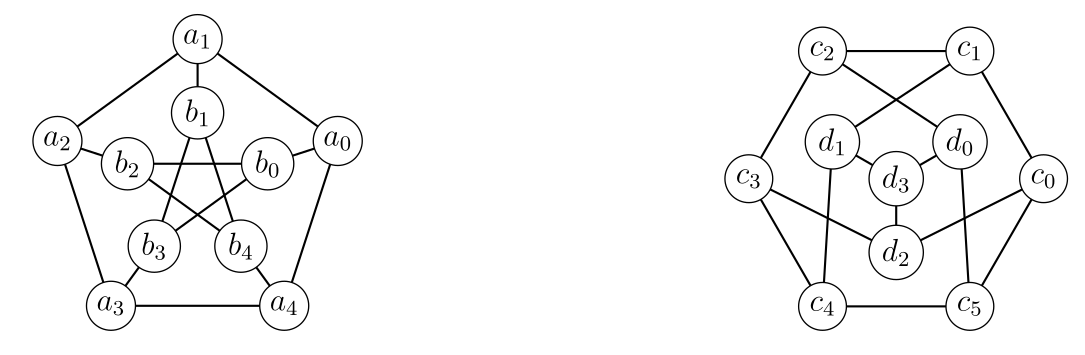
\includegraphics[width=1.0\textwidth]{q8.png}
    \end{figure}
    
    \item\textsuperscript{*} Um grafo é auto-complementar se é isomorfo ao seu complemento. 
    \begin{enumerate}
        \item Dê um exemplo de um grafo auto-complementar não trivial. 
        \item Prove se $G$ é auto-complementar, então $|V(G)|$ ou $|V(G)|-1$ é múltiplo de 4. 
    \end{enumerate}
    
    \item\textsuperscript{*} 
    \begin{enumerate}
        \item Se $G$ é um grafo de 14 vértices e 25 arestas cujos vértices tem graus 3 ou 5, quantos vértices tem grau 3 e quantos tem grau 5? 
        \item Generalize o raciocínio para um grafo de $n$ vértices e $m$ arestas cujos vértices tem graus $d_{1}$ ou $d_{2}$. 
    \end{enumerate}
    
    \item\textsuperscript{*} Prove que se $G$ é um grafo satisfazendo $\delta(G)>0$, $|E(G)|<|V(G)|$, então $G$ tem (pelo menos) dois vértices de grau 1. 
    
    \item\textsuperscript{*} Para todo $n\ge0$ o n-cubo é o grafo definido segue. O 0-cubo é o grafo trivial. Para cada $n>0$ o n-cubo é o grafo obtido colocando-se lado a lado duas cópias do $(n-1)$-cubo e ligando cada vértice de uma das cópias ao seu correspondente na outra cópia. 
    \begin{enumerate}
        \item Desenhe um n-cubo para $n\in\{1,2,3,4\}$ 
        \item Quantos vértices tem um n-cubo? Justifique. 
        \item Quantas arestas tem um n-cubo? Justifique. 
    \end{enumerate}
\end{enumerate}